\documentclass[../rapport.tex]{subfiles}

\begin{document}

\subsubsection{Application 1}

\subsubsection{Use cases de l'application 1}
	\begin{figure}[h!]
		\centering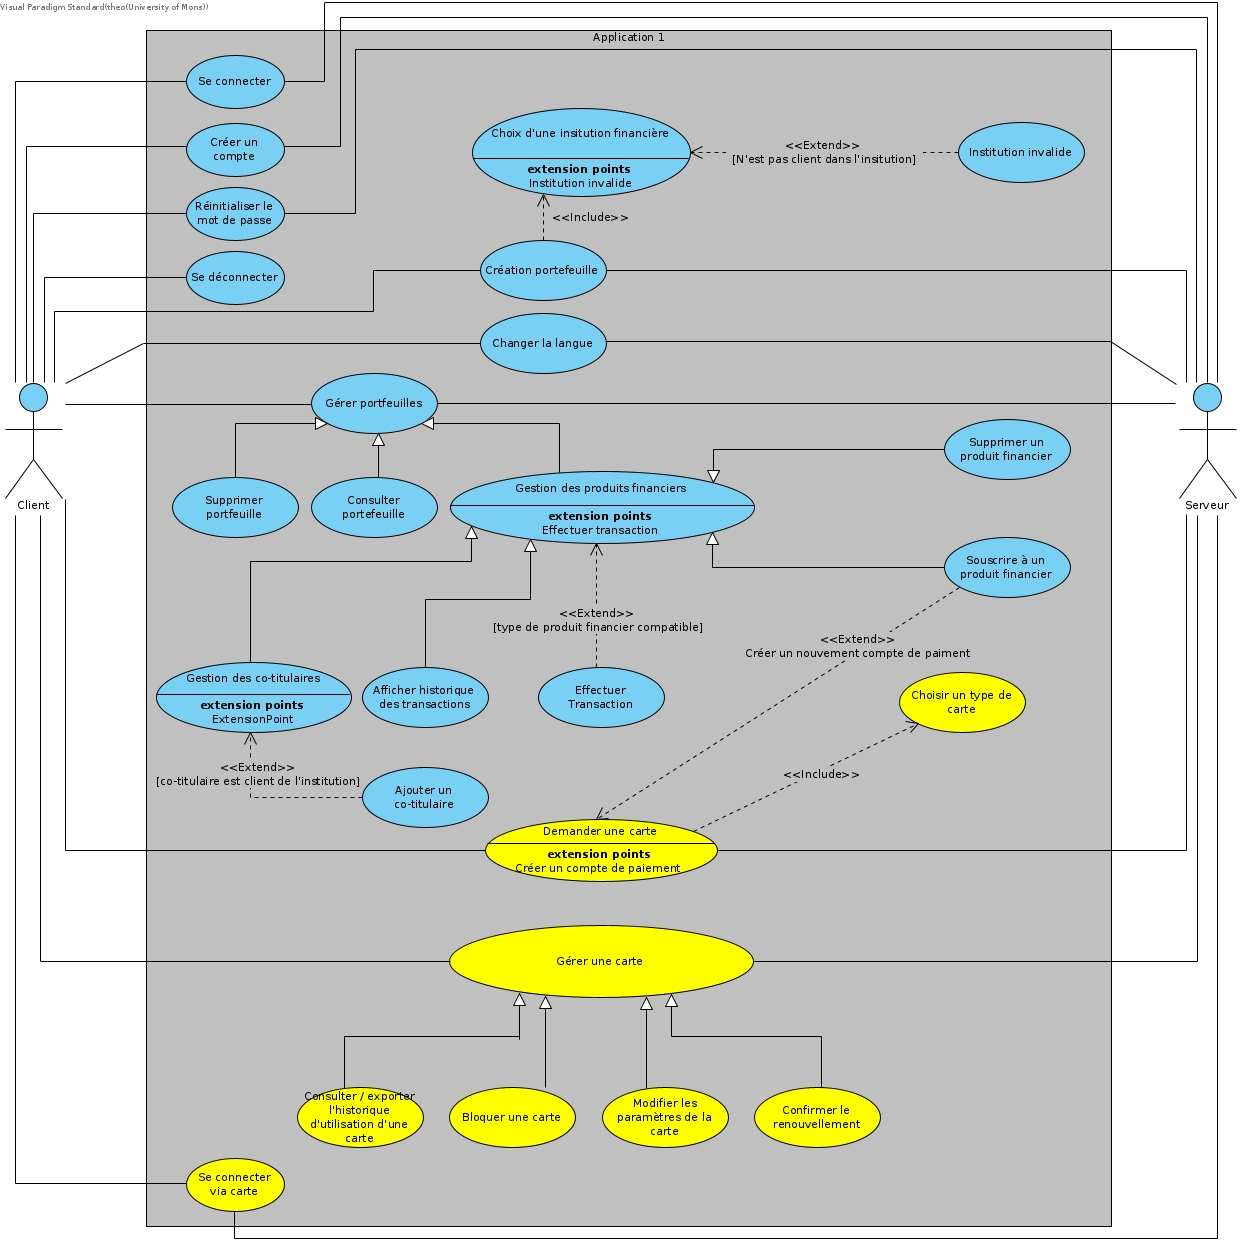
\includegraphics[scale=0.15]{ressources/photos_diagrammes/extensionTheo/diagrams1/useCases1.jpg}
		\caption{Use cases de l'application 1}
	\end{figure}

Les principaux use cases ajoutés afin de supporter les cartes de paiement sont ajouter une carte, gérer une carte et se connecter avec une carte.

\subsubsection{Interaction overview de l'application 1}
	\begin{figure}[h!]
		\centering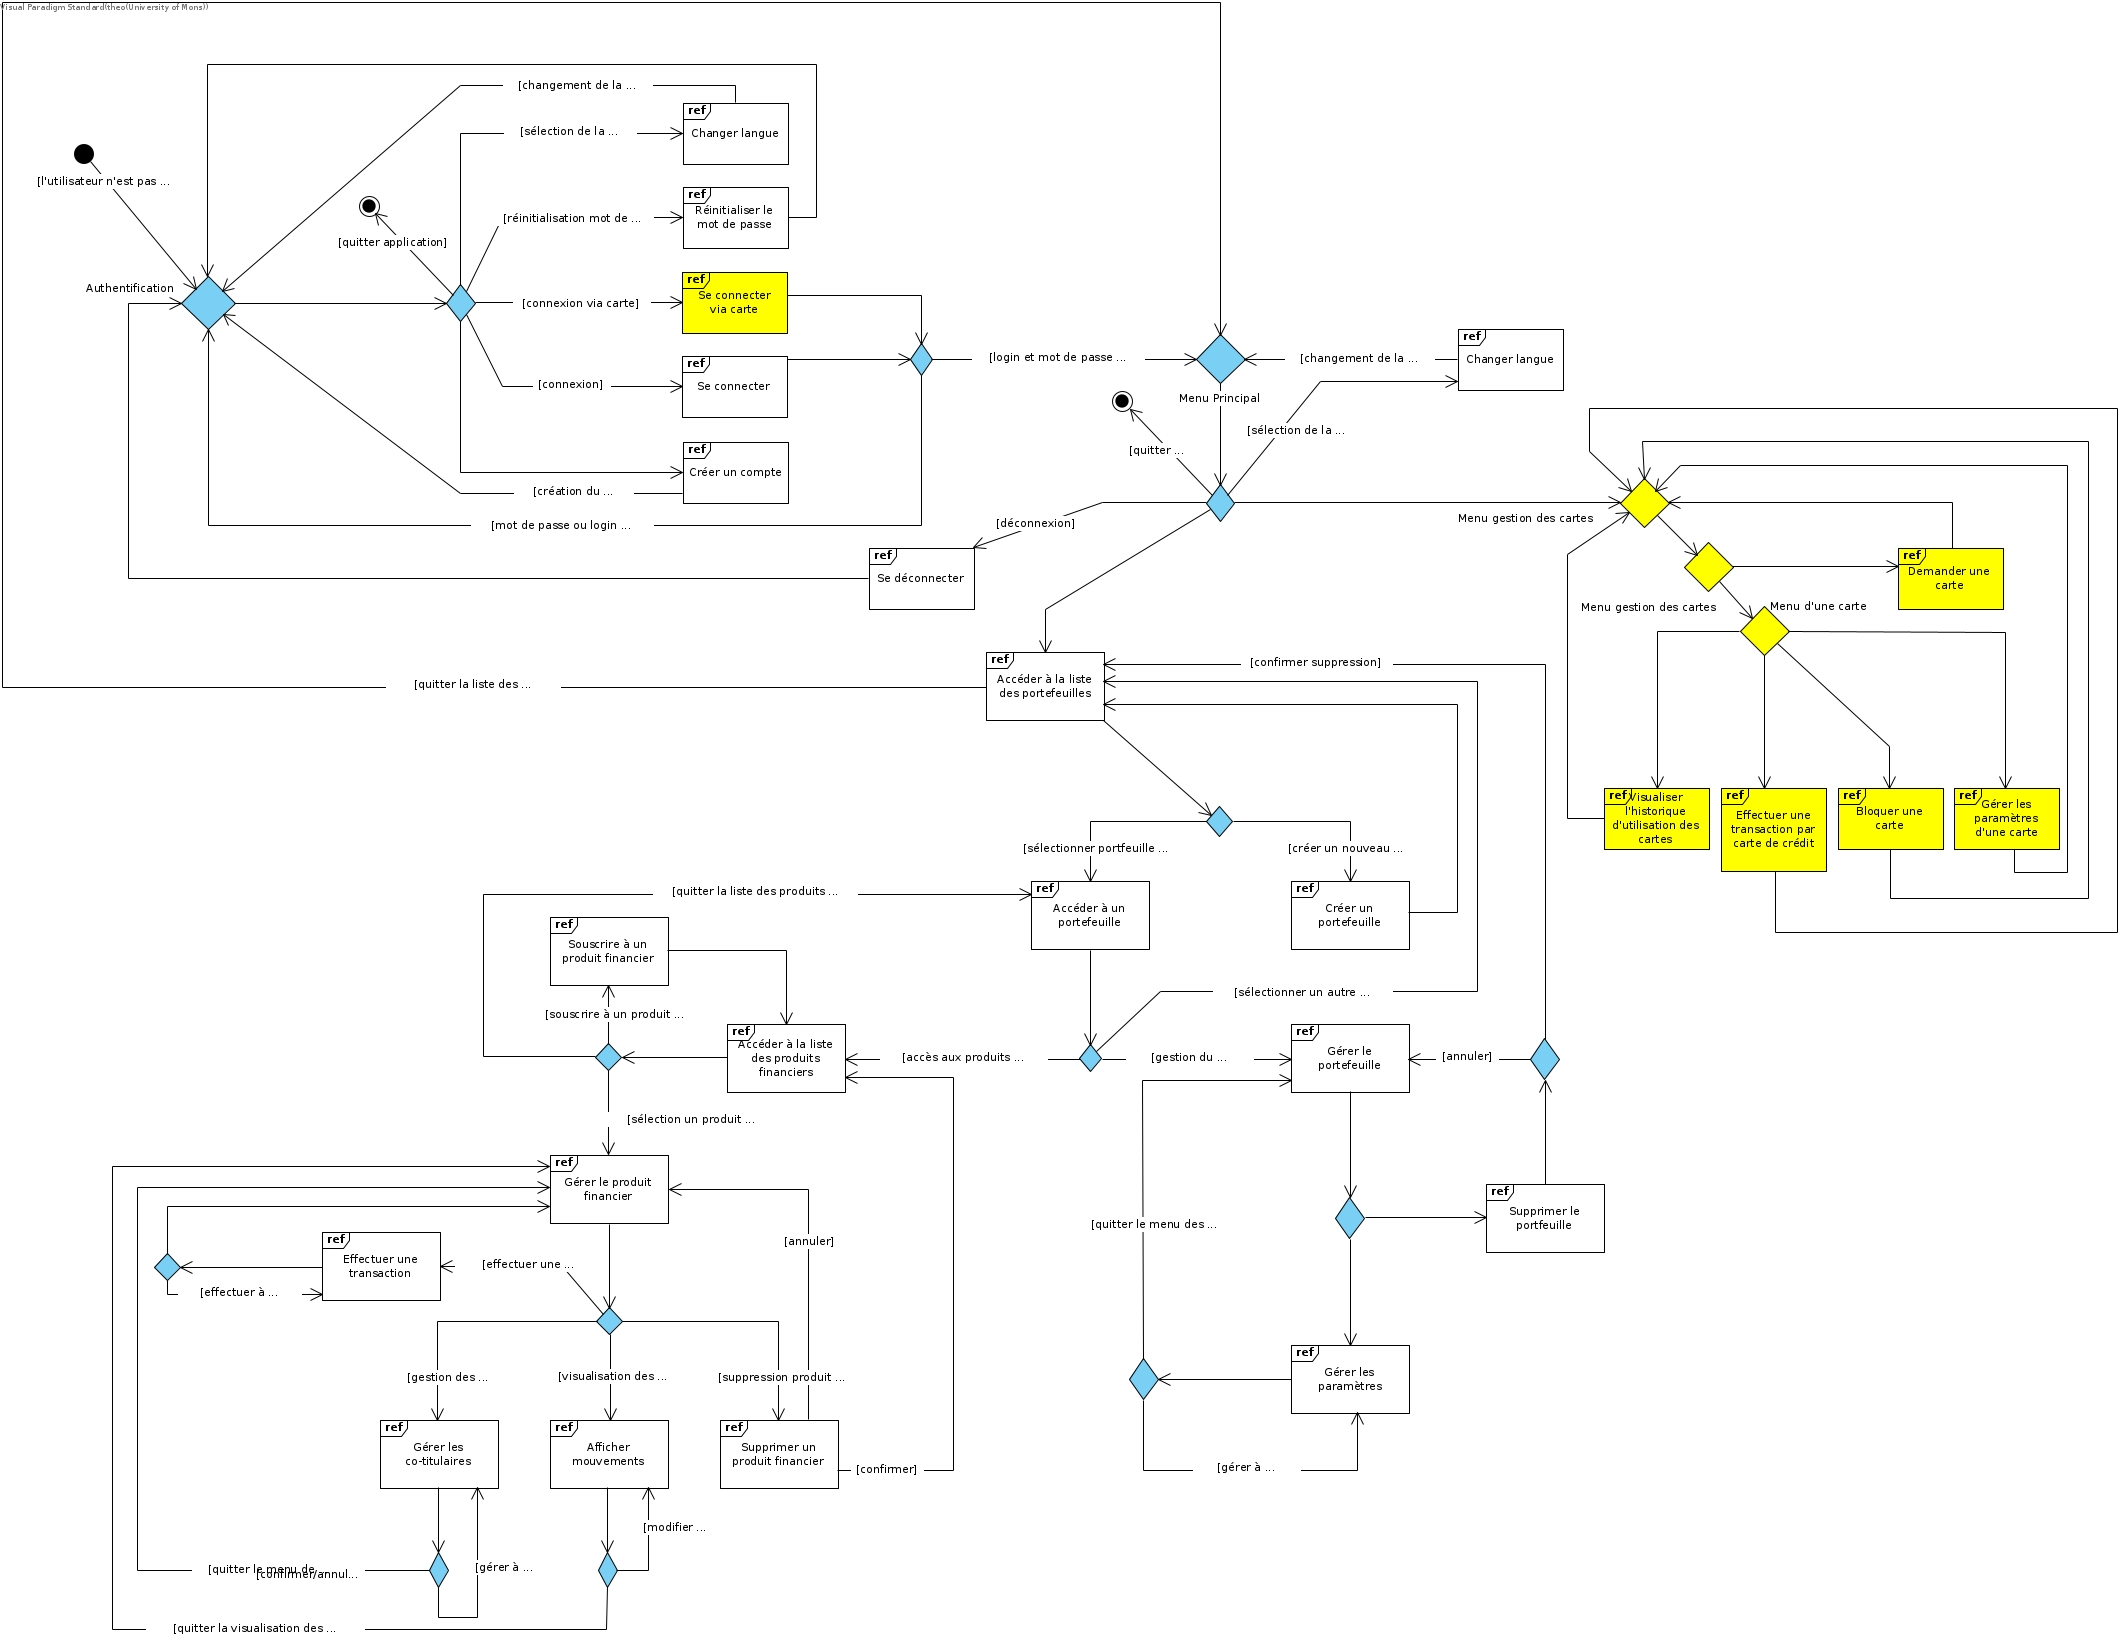
\includegraphics[scale=0.15]{ressources/photos_diagrammes/extensionTheo/diagrams1/InteractionOverviewDiagram1.jpg}
		\caption{Interaction overview diagram de l'application 1}
	\end{figure}

Les use cases de gestion de cartes ont été ajouté au diagramme d'interaction.
Ils sont accessibles via le menu des cartes disponibles dans le menu principal.\\

\subsubsection{Diagramme de classes de l'application 1}
	\begin{figure}[h!]
		\centering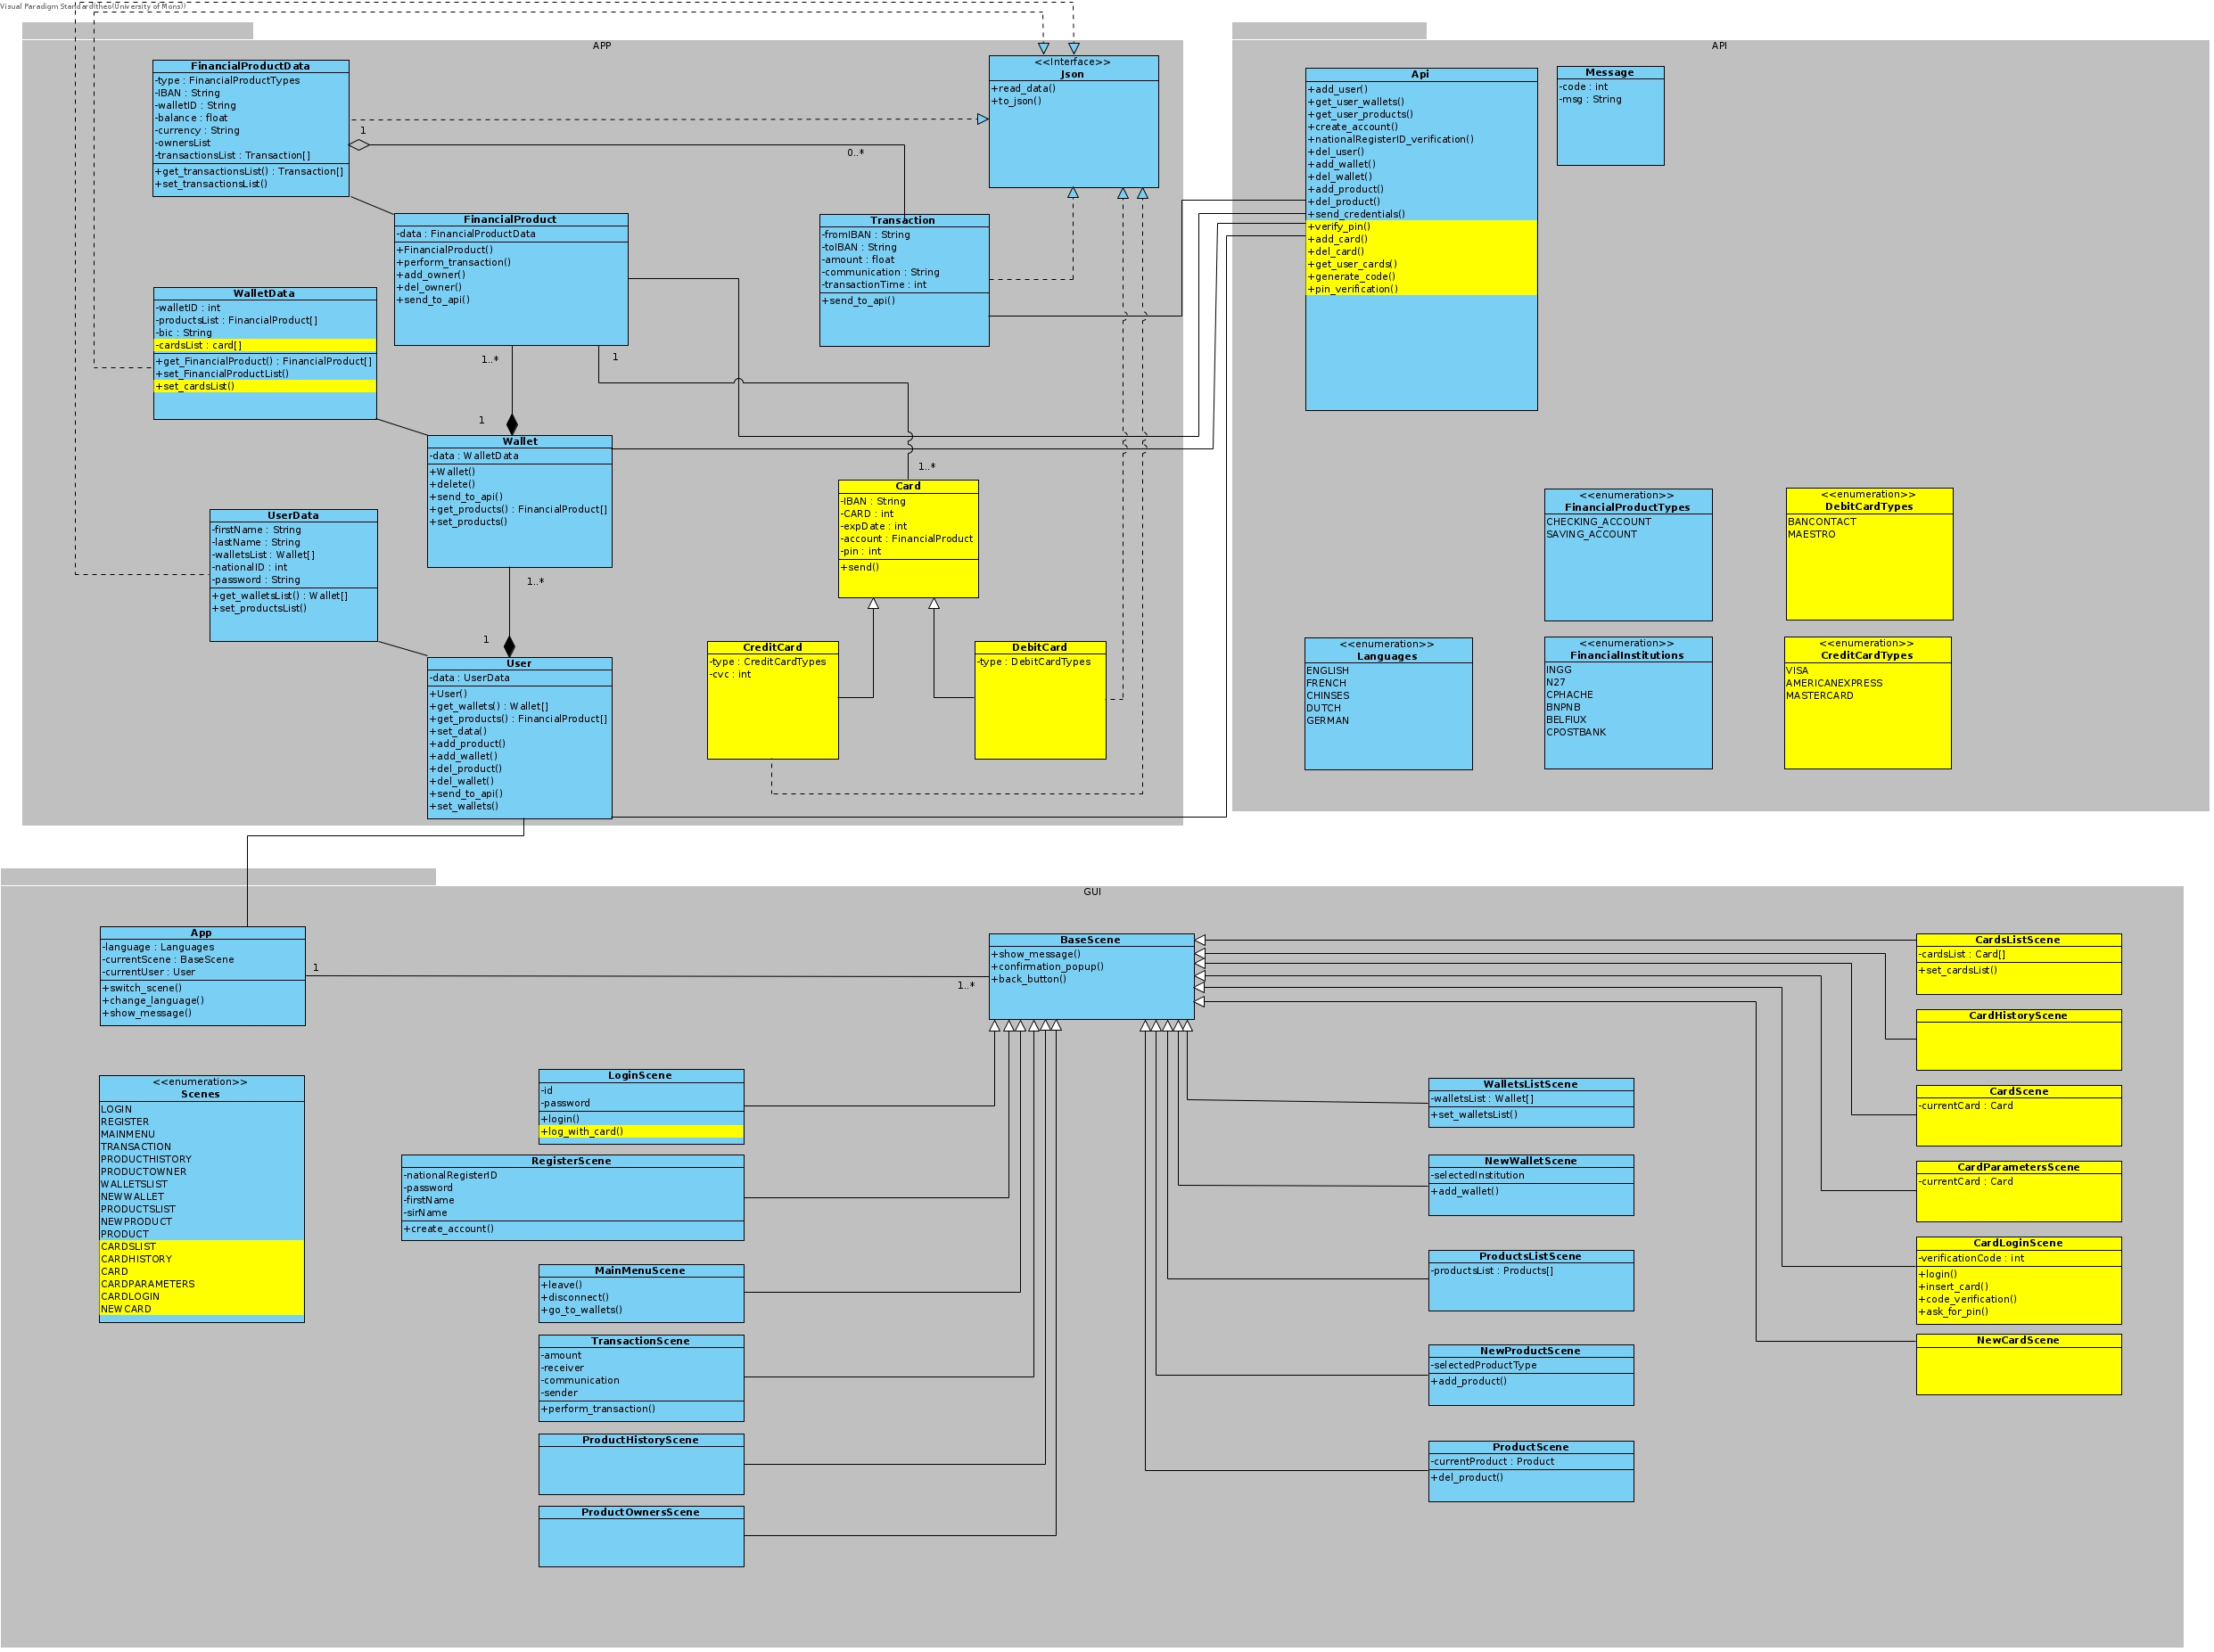
\includegraphics[scale=0.15]{ressources/photos_diagrammes/extensionTheo/diagrams1/classDiagram1.jpg}
		\caption{Class diagram de l'application 1}
	\end{figure}

Dans le package APP, des classes représentant les différents types de cartes ont été ajoutées. Les cartes de débits et de crédits partagent la même classe mère représentant une carte de paiement.\\

Plusieurs scènes ont été ajoutées à l'interface graphique afin de proposer à l'utilisateur des menus de gestion de ses cartes de paiement.\\

\subsubsection{Diagrammes de séquences de l'application 1}
\begin{enumerate}
	\item{Se connecter via une carte}\\
	\begin{figure}[h!]
		\centering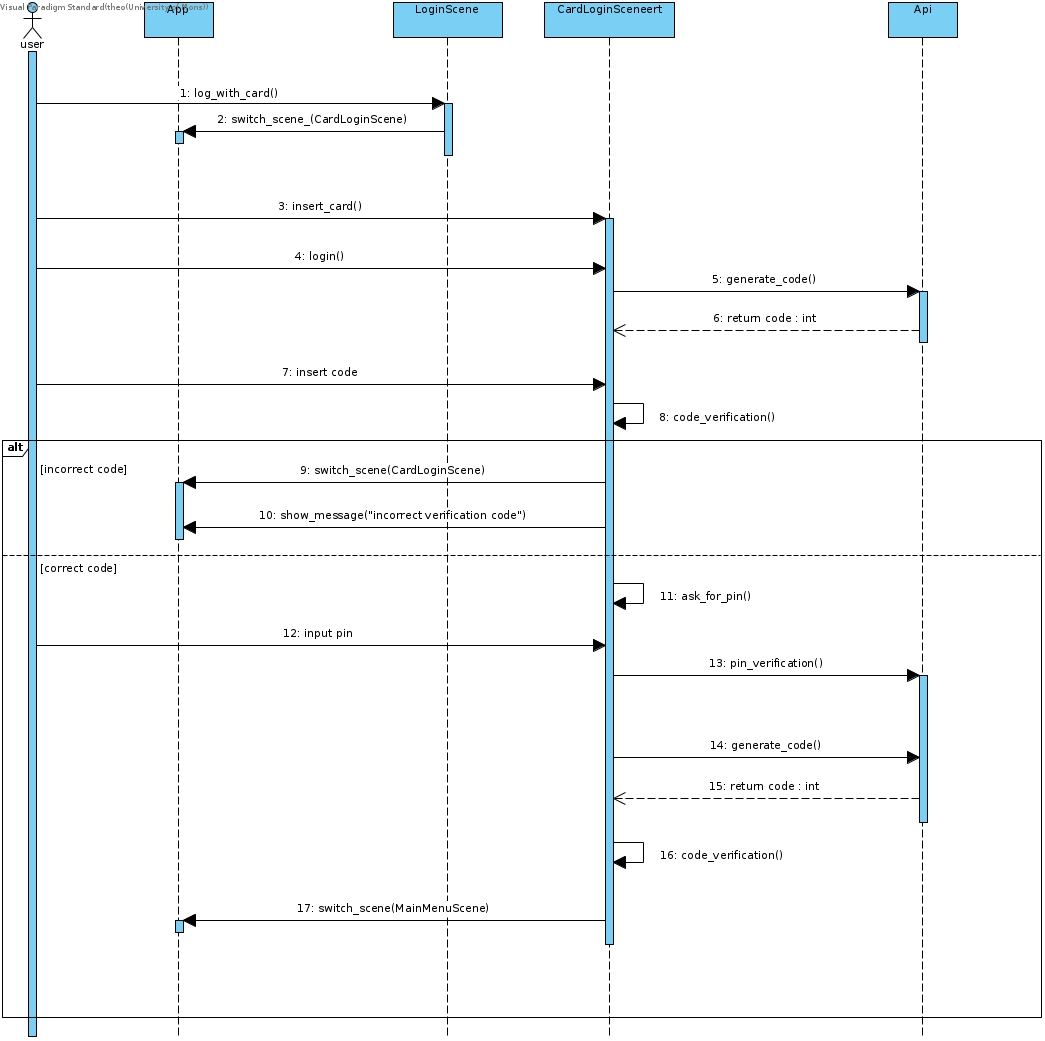
\includegraphics[scale=0.15]{ressources/photos_diagrammes/extensionTheo/diagrams1/seConnecterViaCarte.jpg}
		\caption{Se connecter via une carte}
	\end{figure}\\

Afin de se connecter avec une carte, l'utilisateur doit insérer sa carte dans le lecteur de carte.
Il clique ensuite sur login  et entre le code affiché par l'application. Ce code est  généré via une méthode de l'api.
Il entre ensuite son code pin. Si l'autentification est validée, le lecteur affiche une code qui permettra à l'utilisateur de se connecter à l'application.\\
\end{enumerate}

\subsubsection{Interface graphique de l'application 1}
\begin{enumerate}
	\item{addCardScreen}\\
	\begin{figure}[h!]
		\centering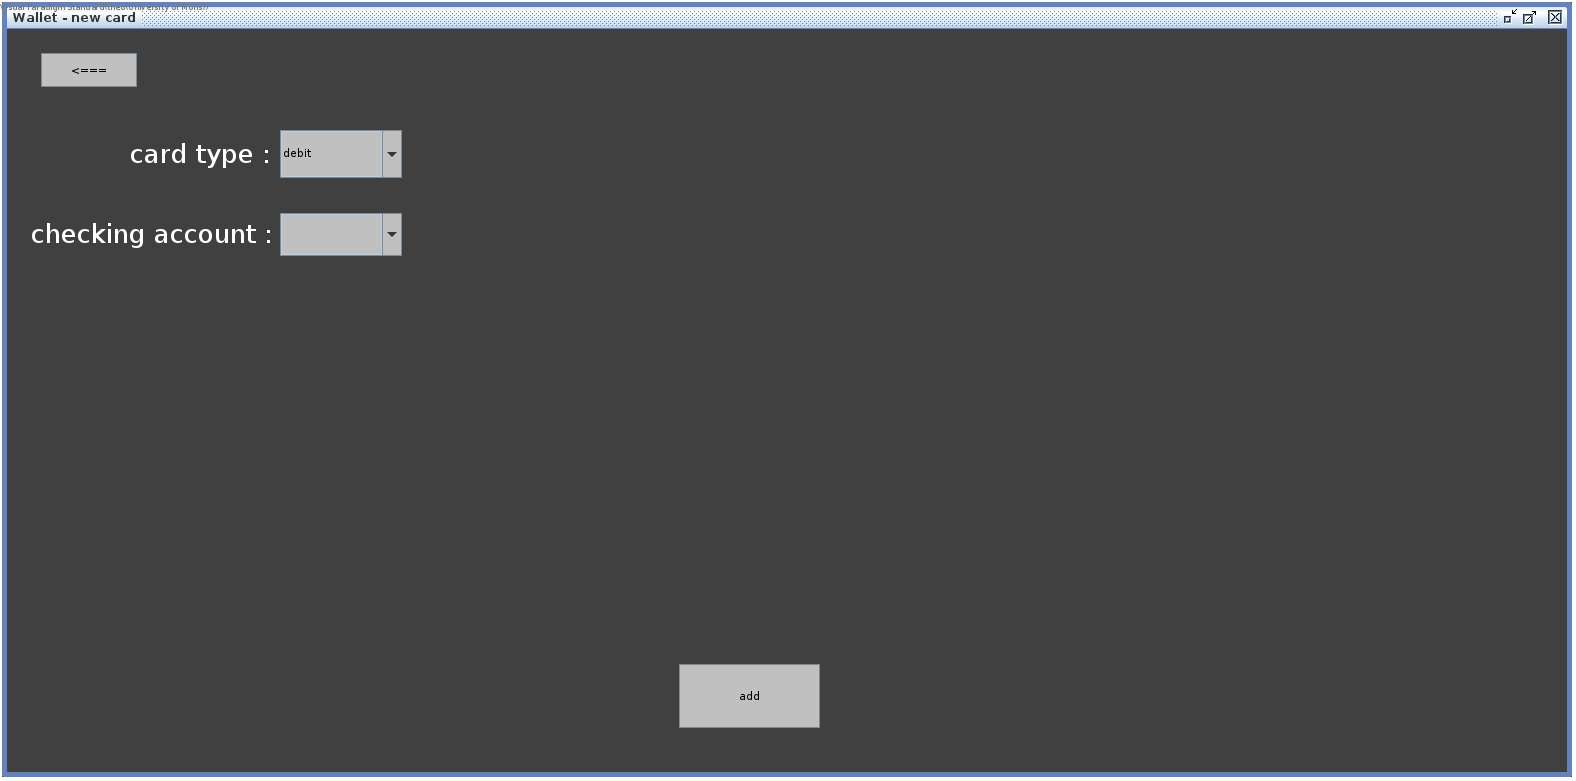
\includegraphics[scale=0.15]{ressources/photos_diagrammes/extensionTheo/gui1/addCard.jpg}
		\caption{Écran d'ajout de carte}
	\end{figure}\\

	\item{cardLoginScreen}\\
	\begin{figure}[h!]
		\centering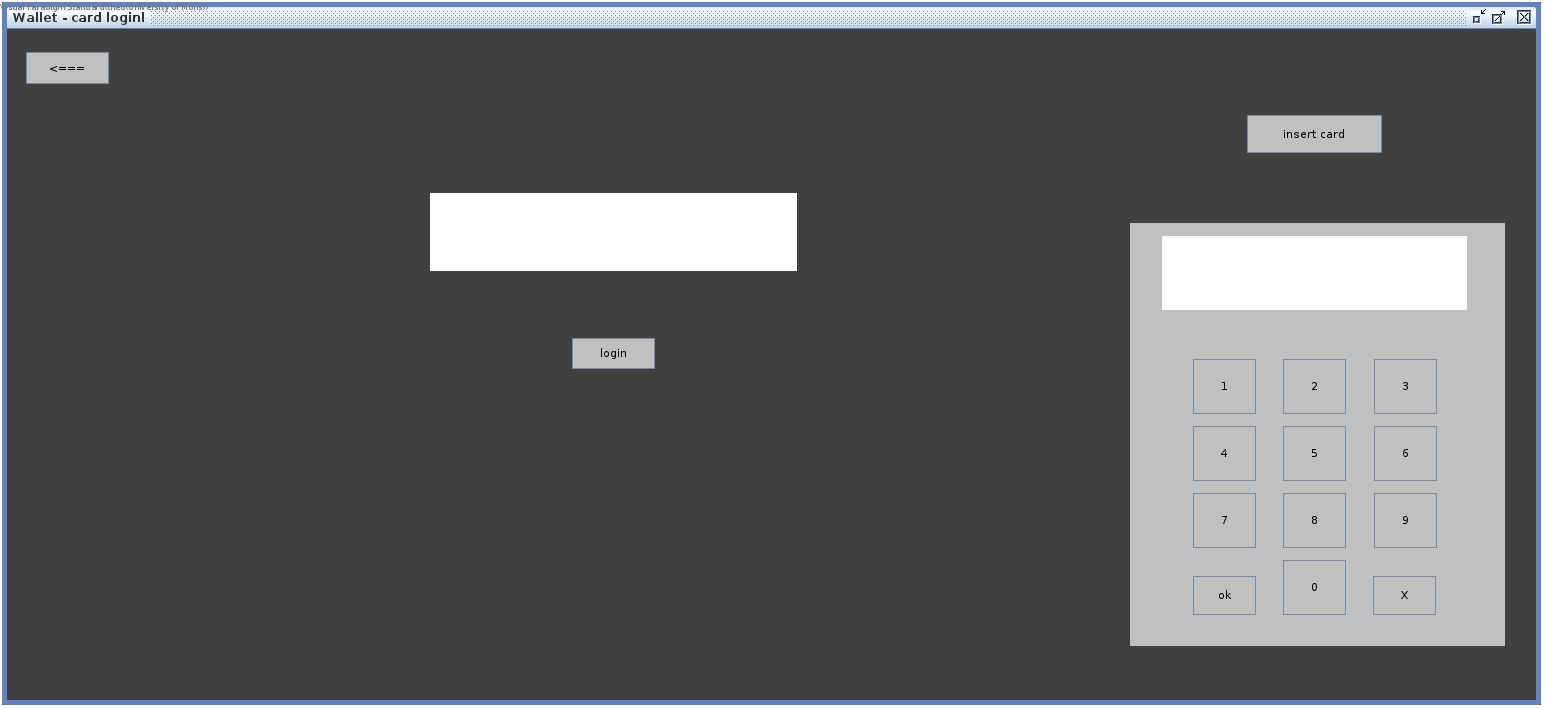
\includegraphics[scale=0.15]{ressources/photos_diagrammes/extensionTheo/gui1/cardLogin.jpg}
		\caption{Écran de connexion via carte}
	\end{figure}\\

Ce menu permet à l'utilisateur de se connecter avec une carte.\\
La partie droite de l'écran représente un lecteur de carte afin de simuler l'insertion d'une carte.

	\item{cardScreen}\\
	\begin{figure}[h!]
		\centering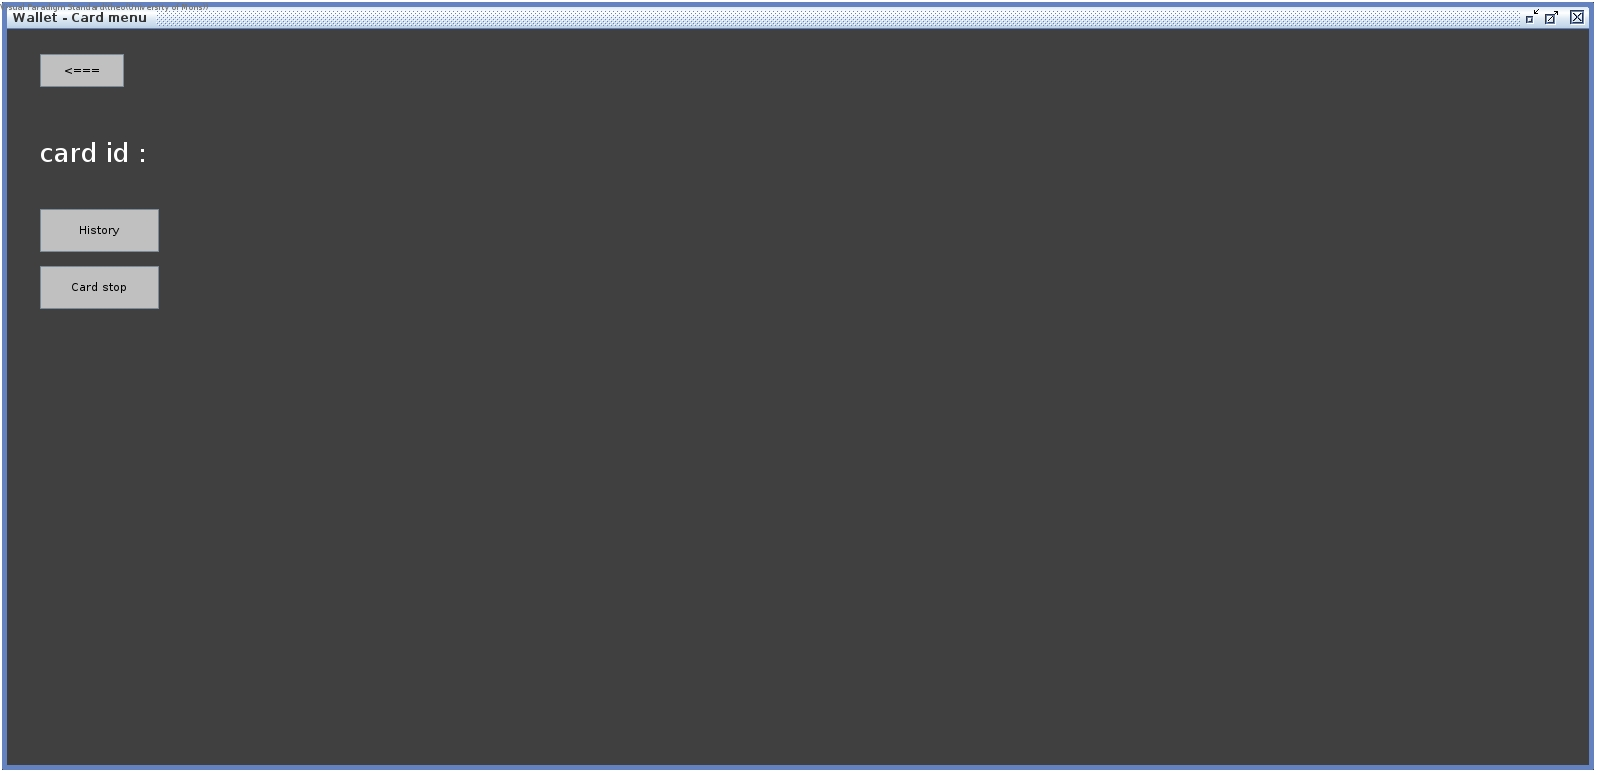
\includegraphics[scale=0.15]{ressources/photos_diagrammes/extensionTheo/gui1/CardScene.jpg}
		\caption{Écran de gestion d'une carte}
	\end{figure}\\

	\item{cardListScreen}\\
	\begin{figure}[h!]
		\centering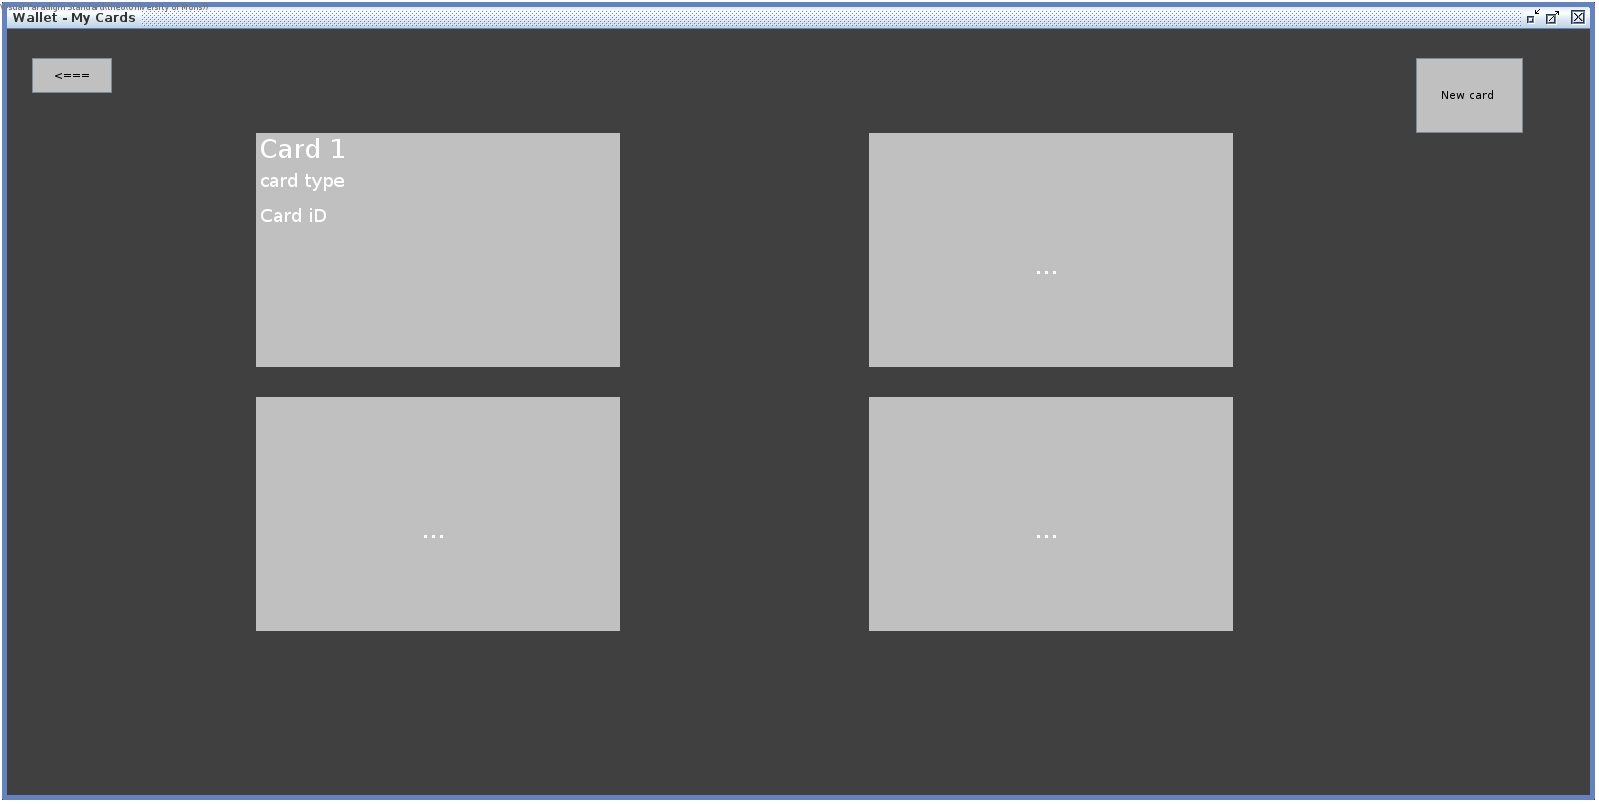
\includegraphics[scale=0.15]{ressources/photos_diagrammes/extensionTheo/gui1/CardsListScreen.jpg}
		\caption{Écran de la liste de cartes}
	\end{figure}\\
Cet écran liste toutes les cartes de l'utilisateur.\\
Il peut cliquer sur n'importe quelle carte afin d'accèder au menu de cette carte.

	\item{cardsParametersScreen}\\
	\begin{figure}[h!]
		\centering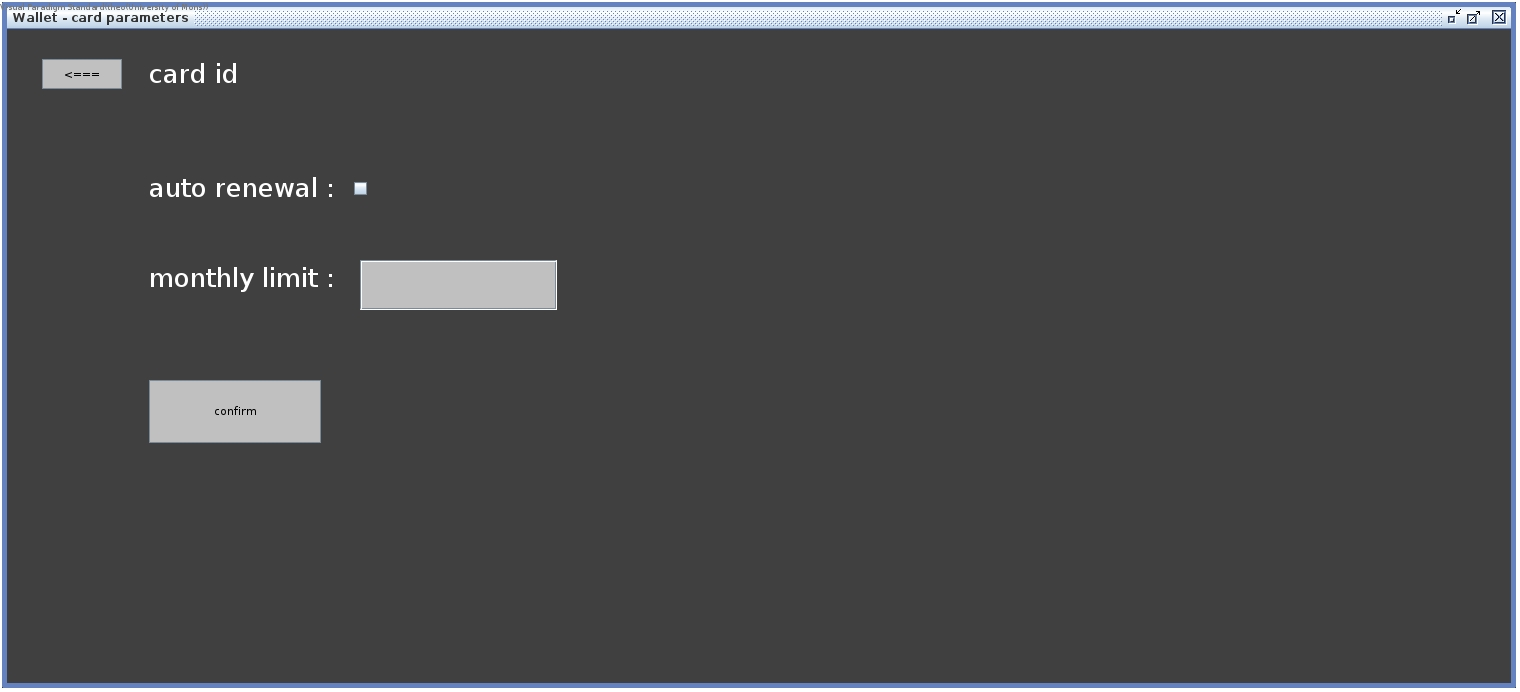
\includegraphics[scale=0.15]{ressources/photos_diagrammes/extensionTheo/gui1/cardsParametres.jpg}
		\caption{Écran de paramètres d'une carte}
	\end{figure}\\
Cet écran permet de modifier les paramètres d'une carte tel que le plafond mensuel et le renouvellement automatique.

	\item{loginScreen}\\
	\begin{figure}[h!]
		\centering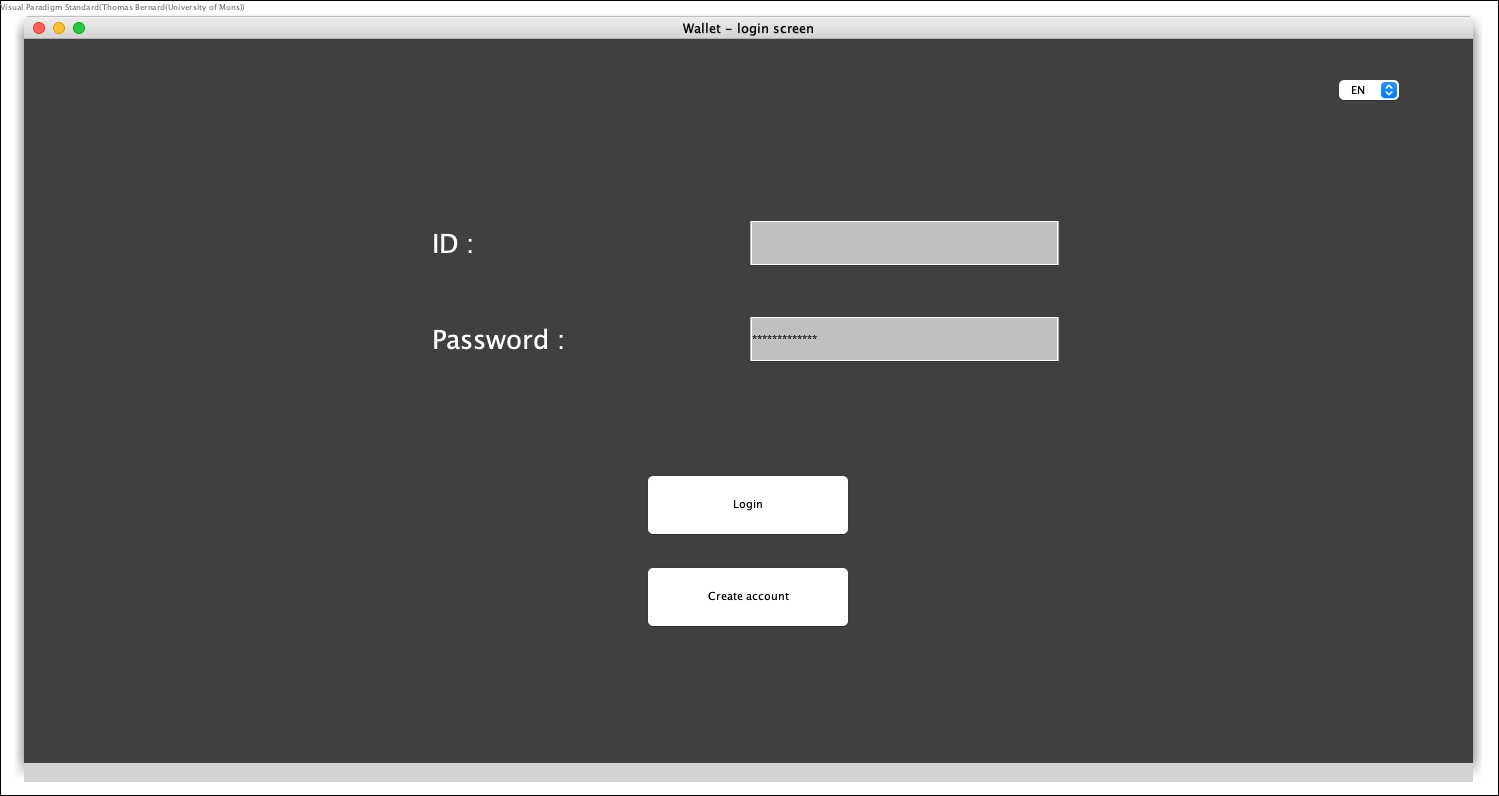
\includegraphics[scale=0.15]{ressources/photos_diagrammes/extensionTheo/gui1/login.jpg}
		\caption{Écran connexion}
	\end{figure}\\
Le bouton ``login with card'' permet à l'utilisateur d'accèder au menu de connexion par carte.

	\item{mainMenuScreen}\\
	\begin{figure}[h!]
		\centering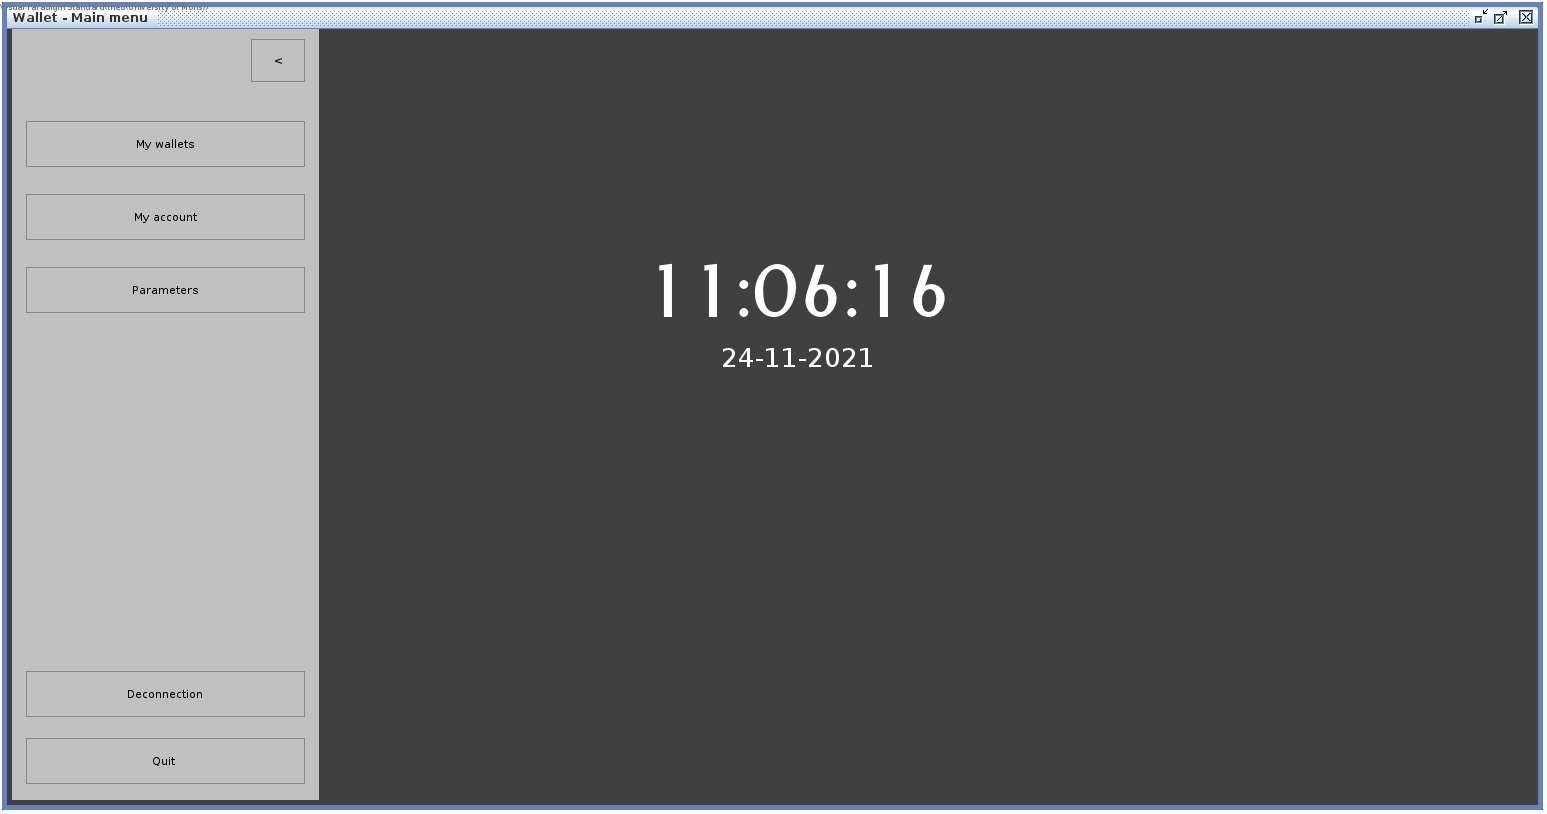
\includegraphics[scale=0.15]{ressources/photos_diagrammes/extensionTheo/gui1/mainMenu.jpg}
		\caption{Écran principal}
	\end{figure}\\

Le bouton ``My cards'' permet à l'utilisateur d'accèder au menu de gestion des cartes.

\end{enumerate}

\subsubsection{Application 2}
\subsubsection{Use cases de l'application 2}
	\begin{figure}[h!]
		\centering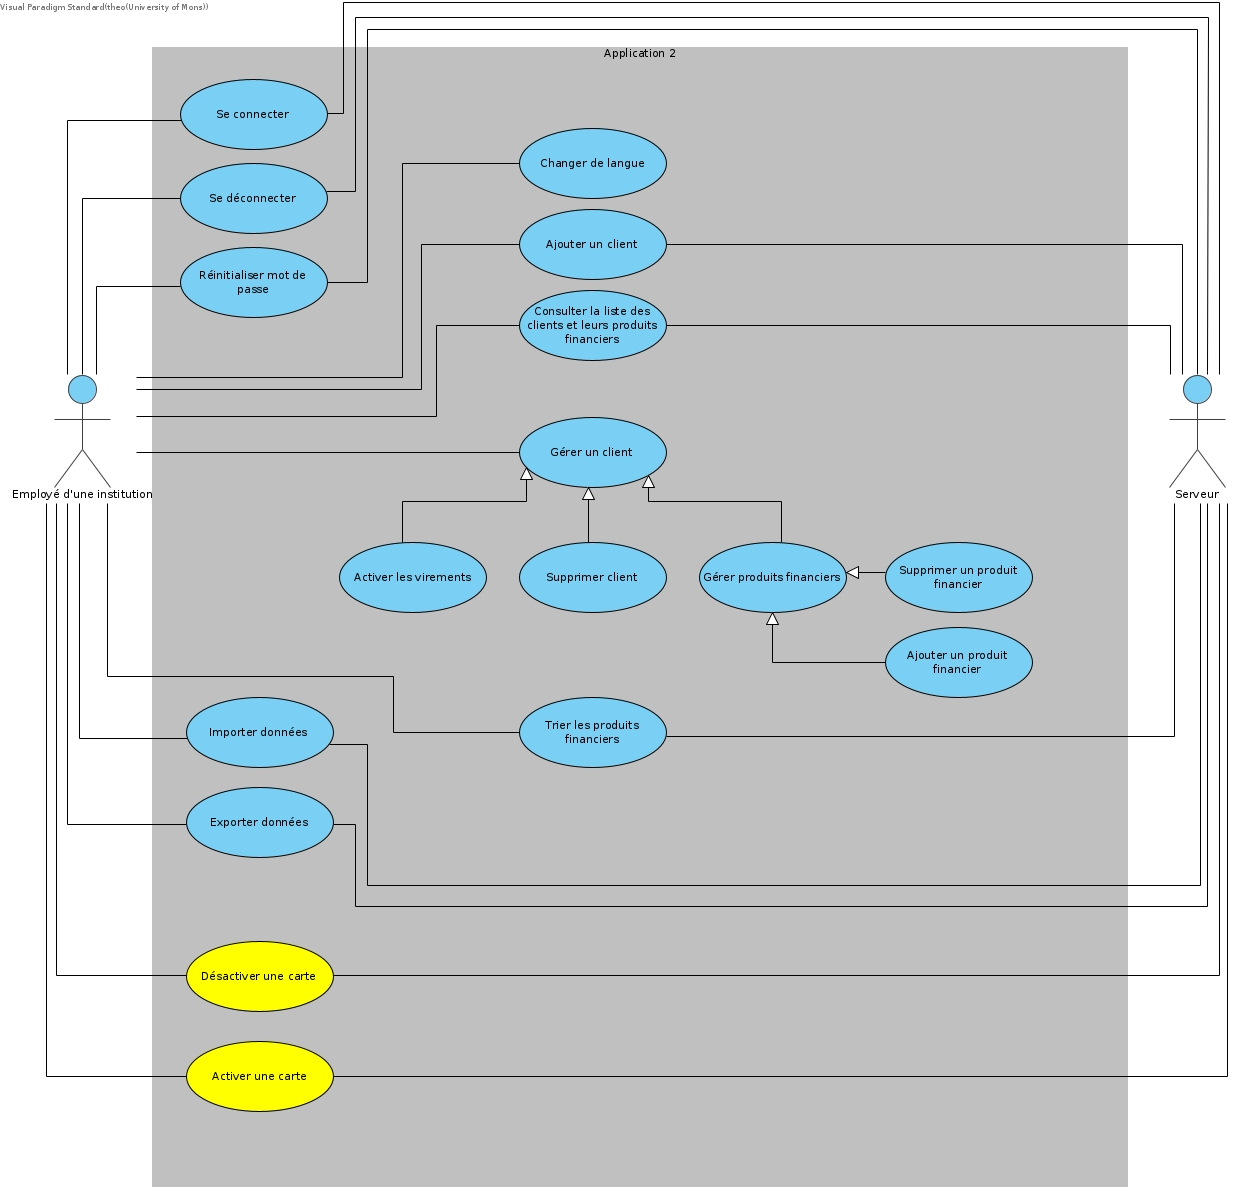
\includegraphics[scale=0.15]{ressources/photos_diagrammes/extensionTheo/diagrams2/useCases2.jpg}
		\caption{Use cases de l'application 2}
	\end{figure}

\subsubsection{Interaction overview de l'application 2}
	\begin{figure}[h!]
		\centering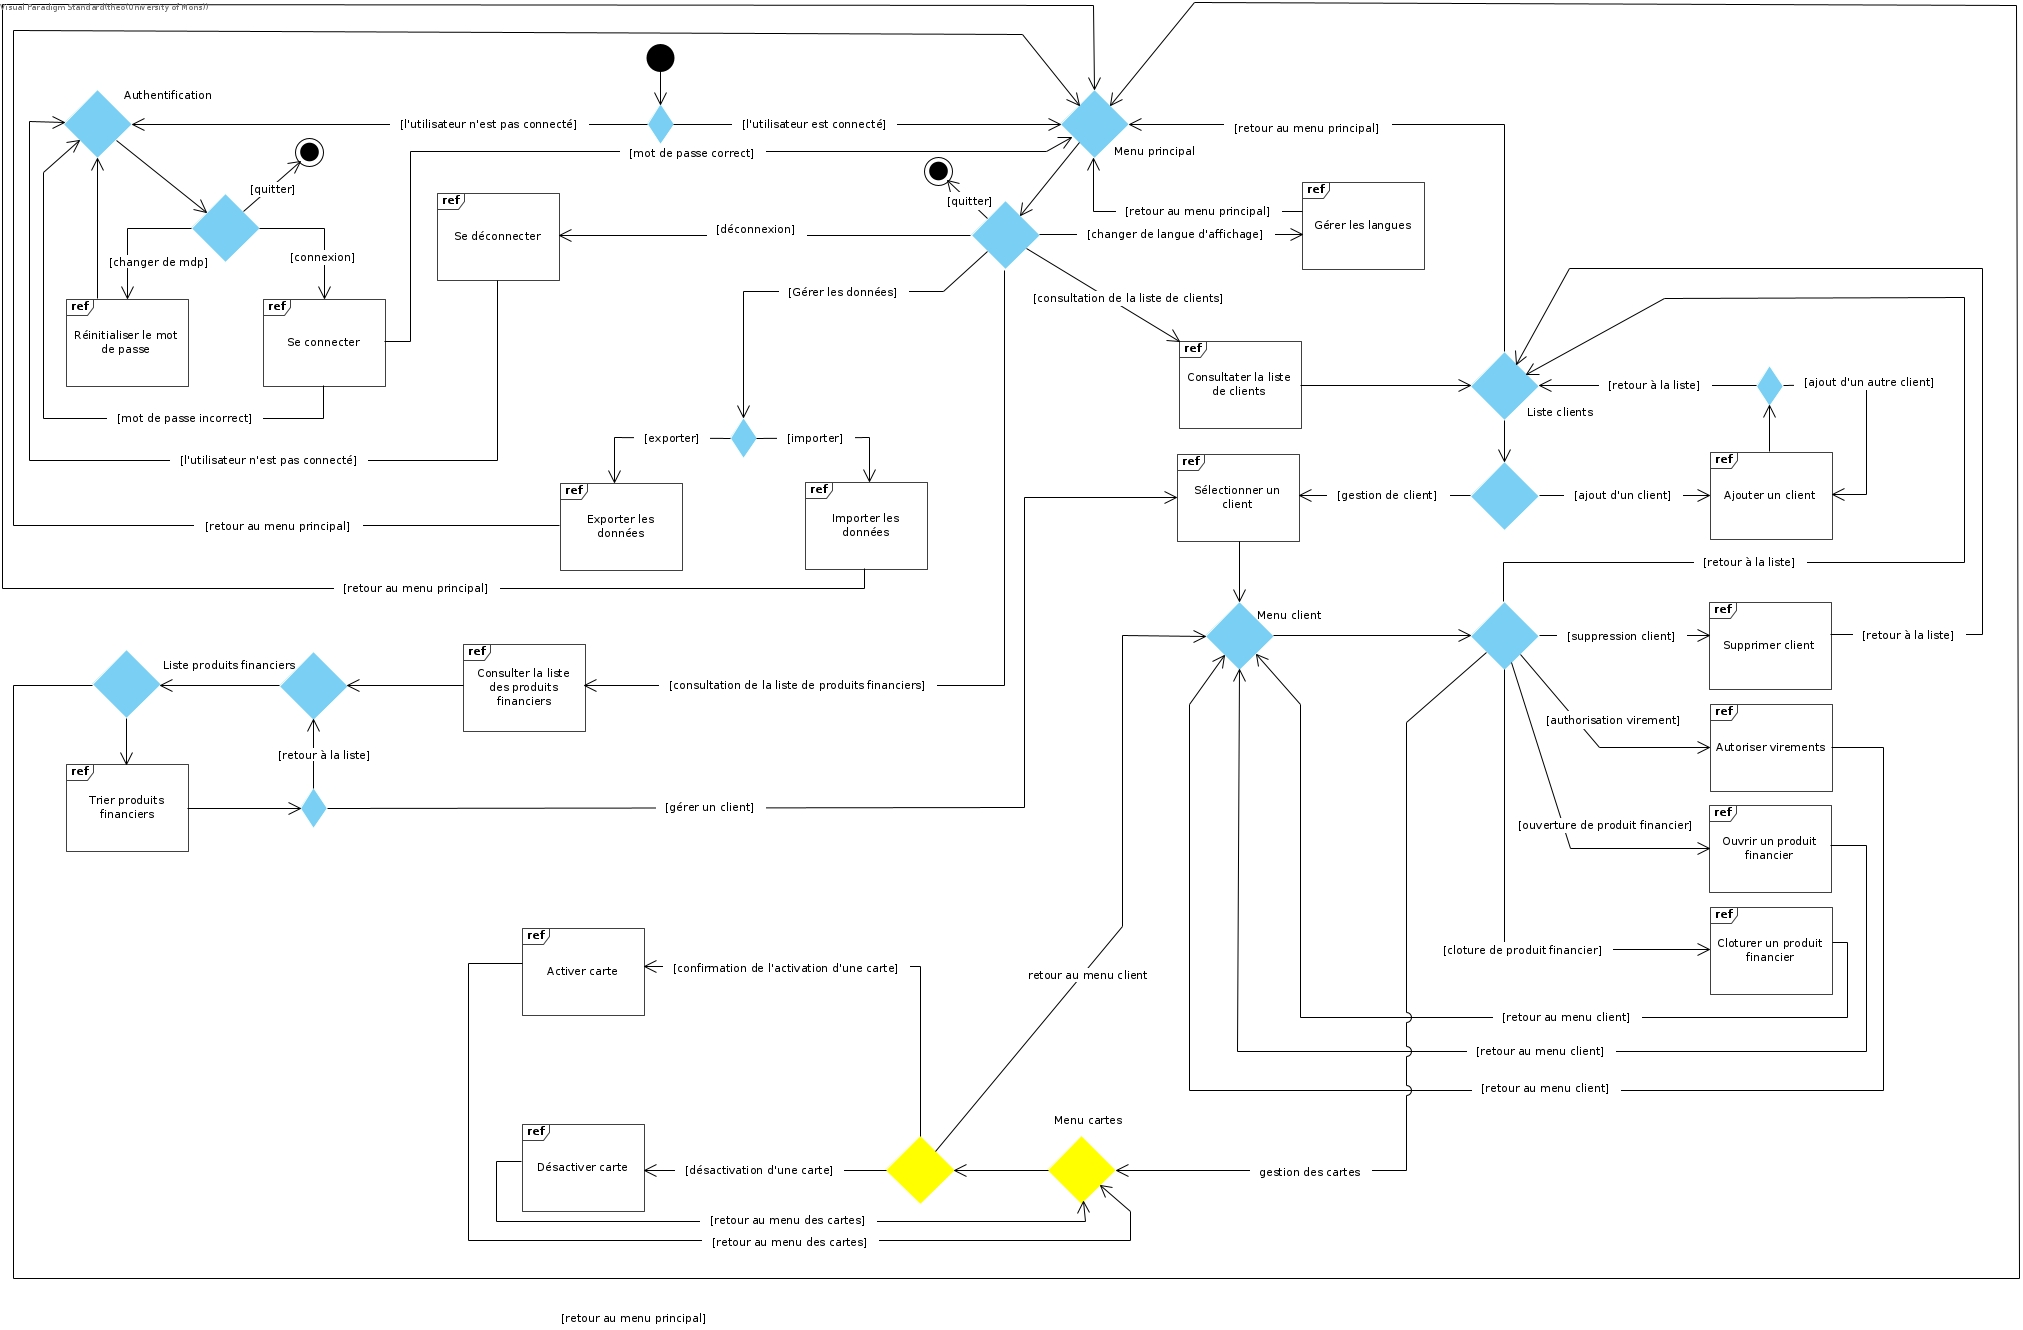
\includegraphics[scale=0.15]{ressources/photos_diagrammes/extensionTheo/diagrams2/interactionOverview2.jpg}
		\caption{Interaction overciew de l'application 2}
	\end{figure}
\subsubsection{Diagramme de classes de l'application 2}
	\begin{figure}[h!]
		\centering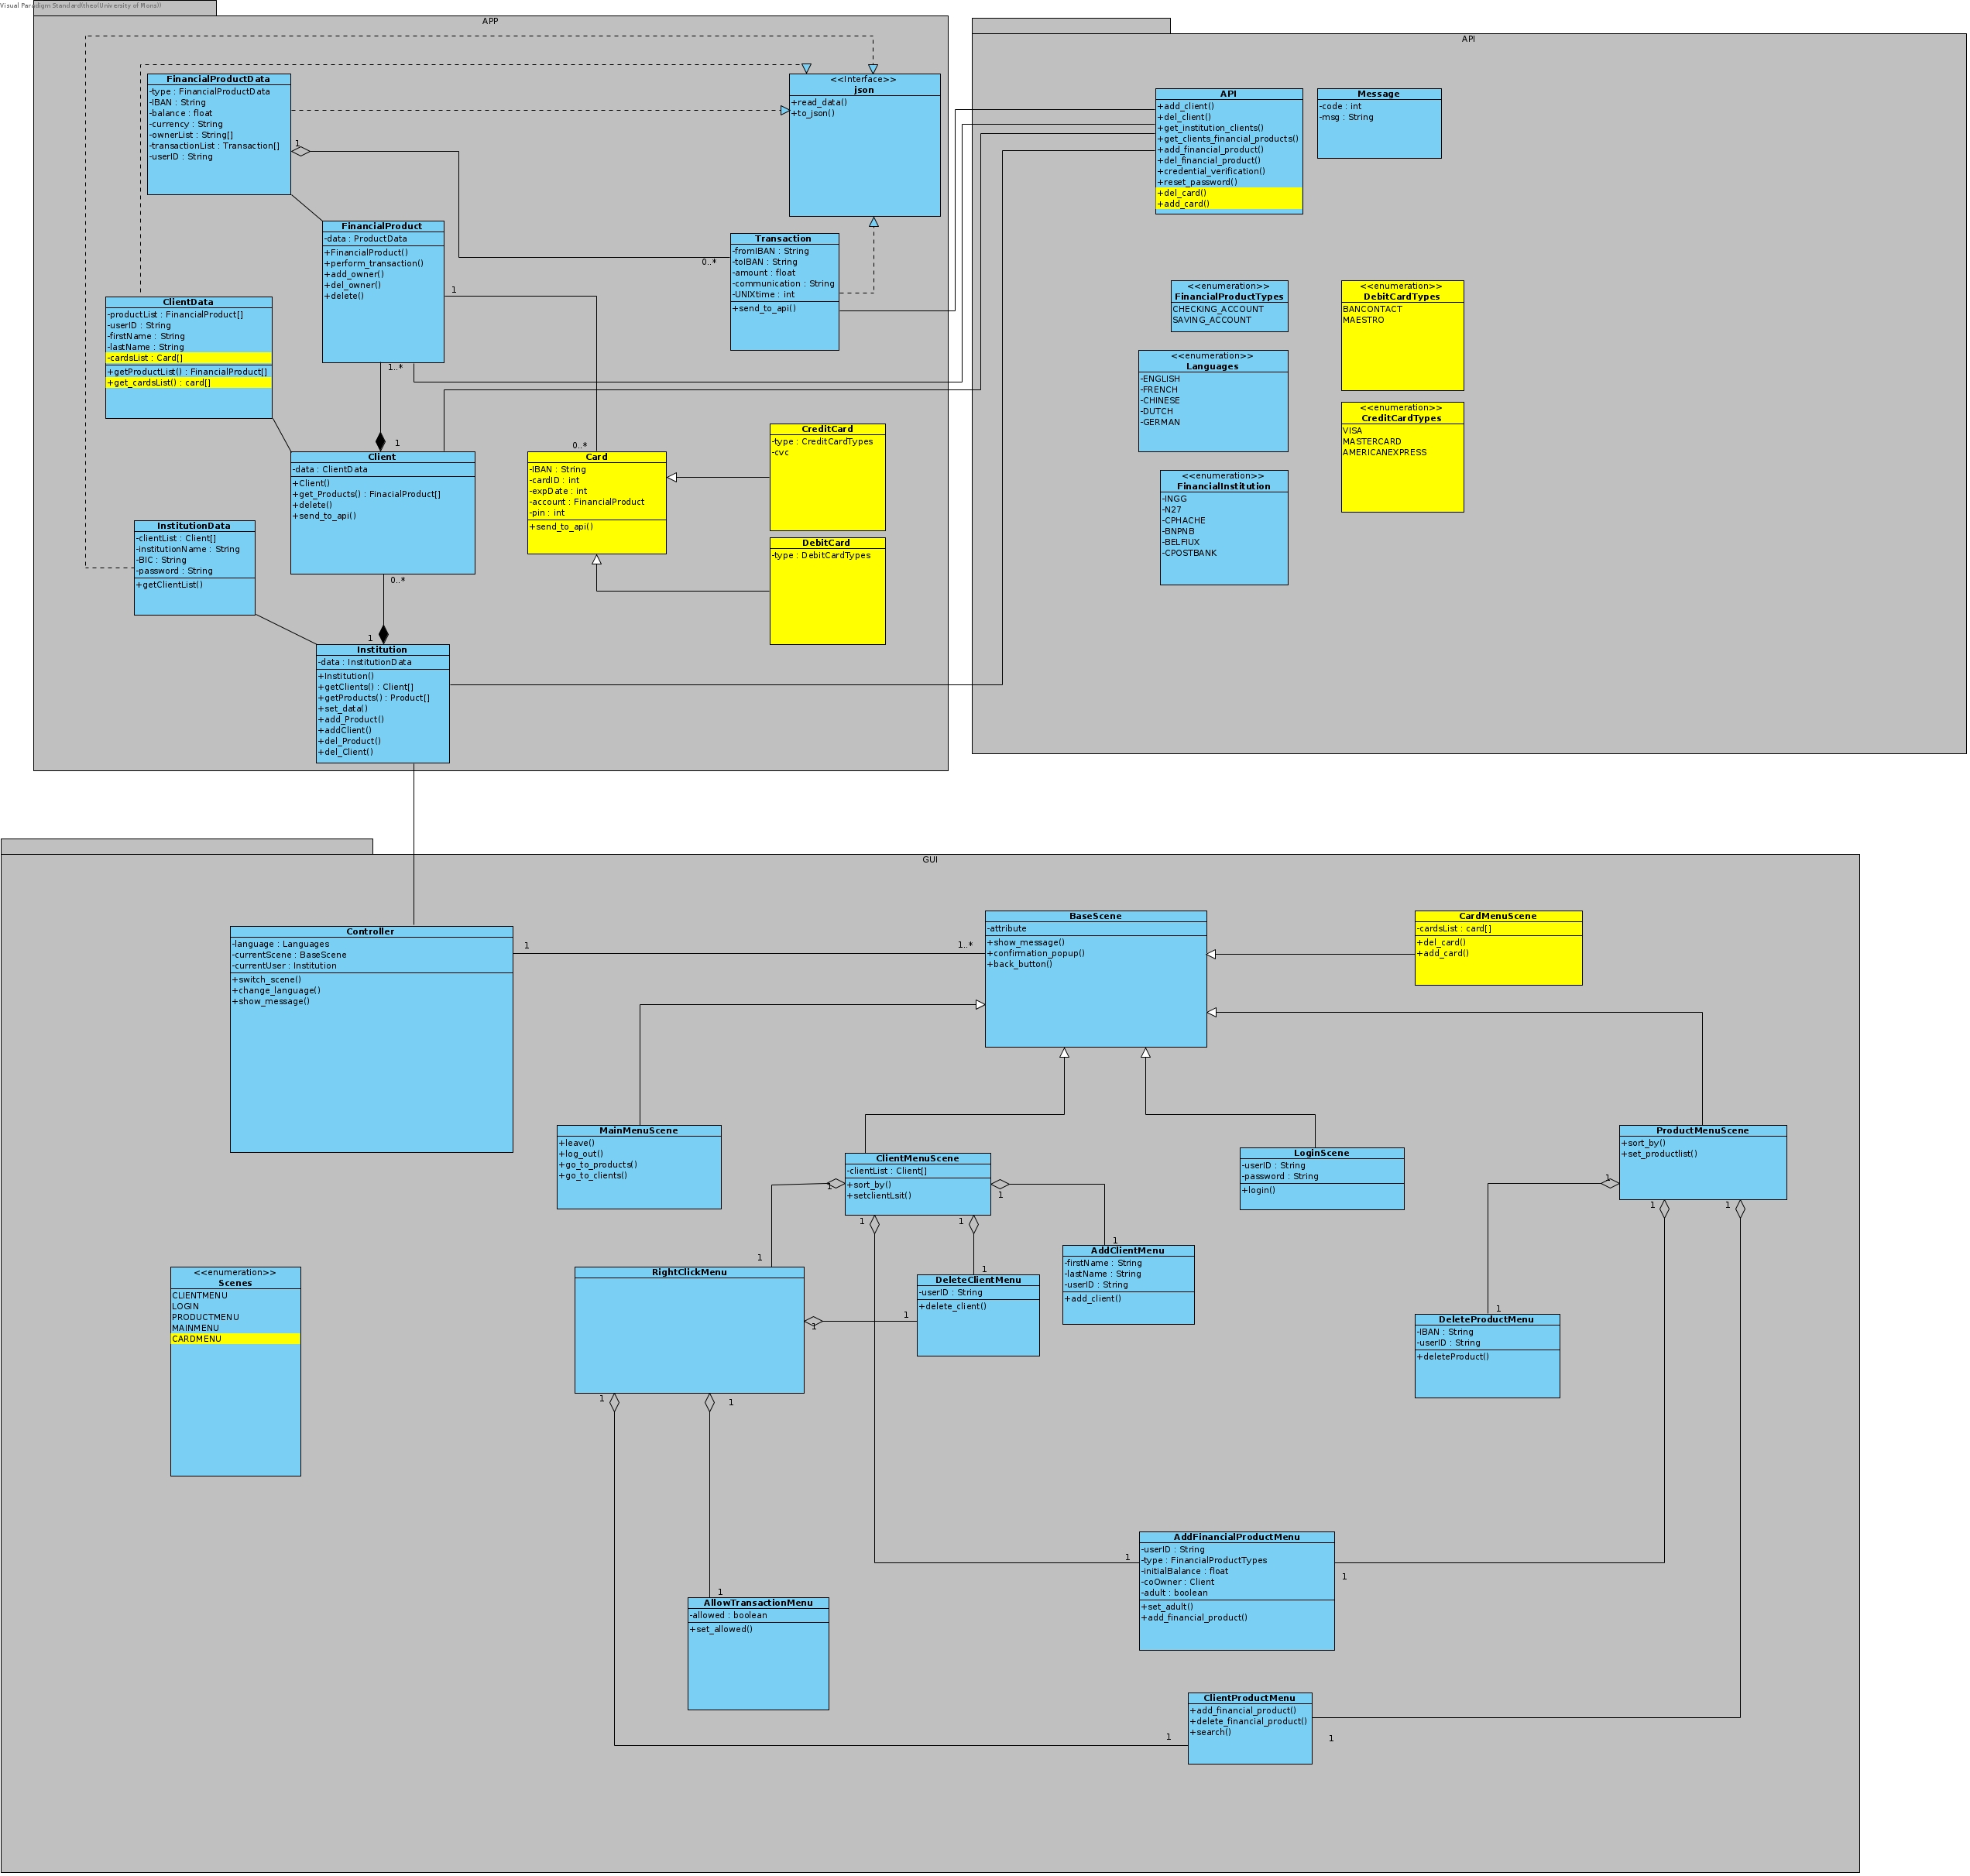
\includegraphics[scale=0.15]{ressources/photos_diagrammes/extensionTheo/diagrams2/classDiagram2.jpg}
		\caption{Interaction overciew de l'application 2}
	\end{figure}

\subsubsection{Interface graphique de l'application 2}
\begin{enumerate}
	\item{CardMenuScreen}\\
	\begin{figure}[h!]
		\centering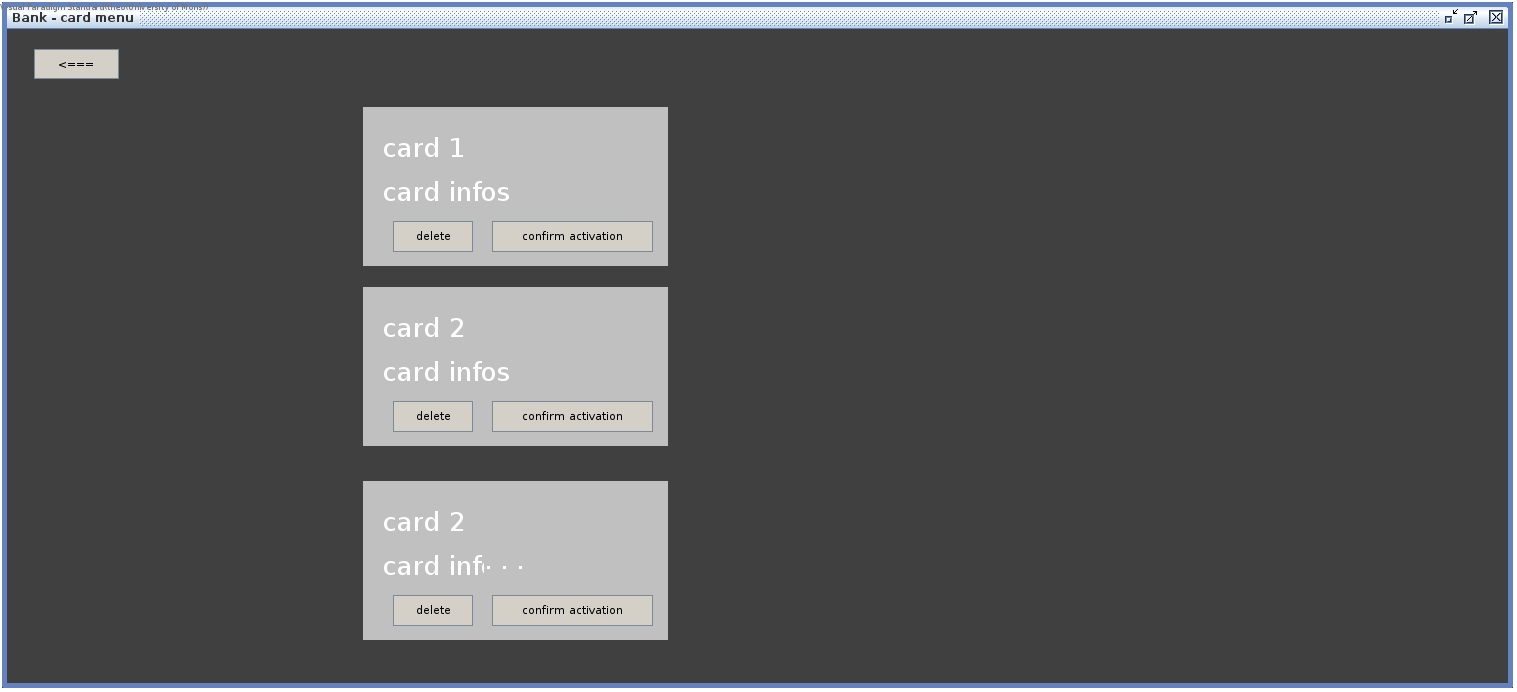
\includegraphics[scale=0.15]{ressources/photos_diagrammes/extensionTheo/gui2/cardMenu.jpg}
		\caption{Écran de gestion des cartes}
	\end{figure}\\

\item{clientProductScreen}\\
	\begin{figure}[h!]
		\centering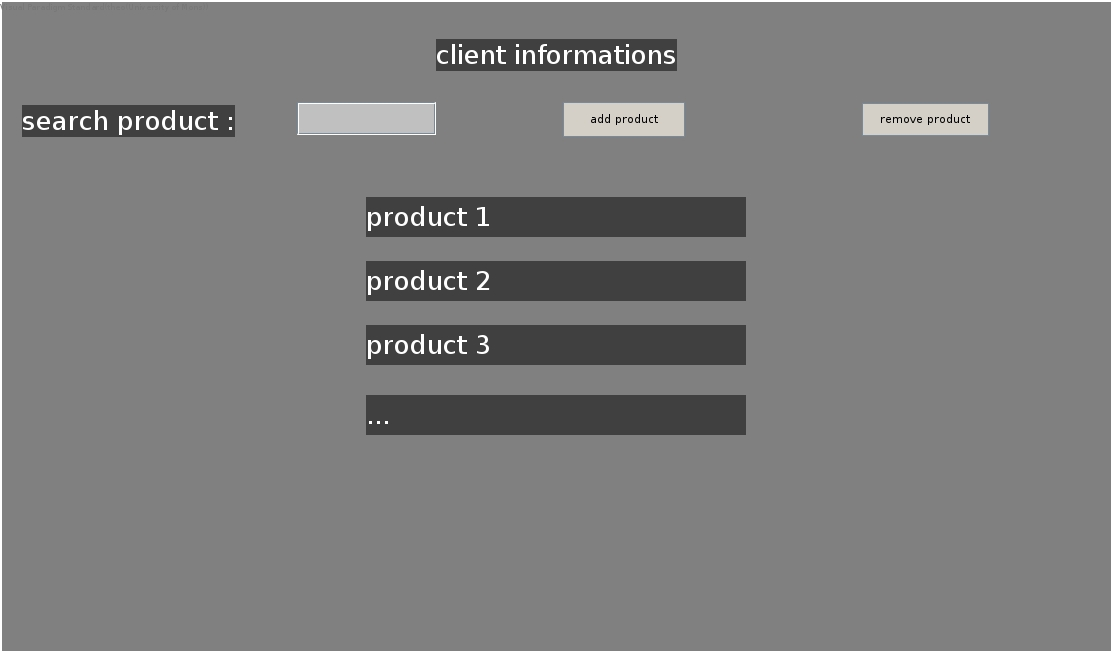
\includegraphics[scale=0.15]{ressources/photos_diagrammes/extensionTheo/gui2/clientProductMenu.jpg}
		\caption{Écran des produits d'un client}
	\end{figure}

\end{enumerate}

\subsubsection{Diagramme d'entité relation}
	\begin{figure}[h!]
		\centering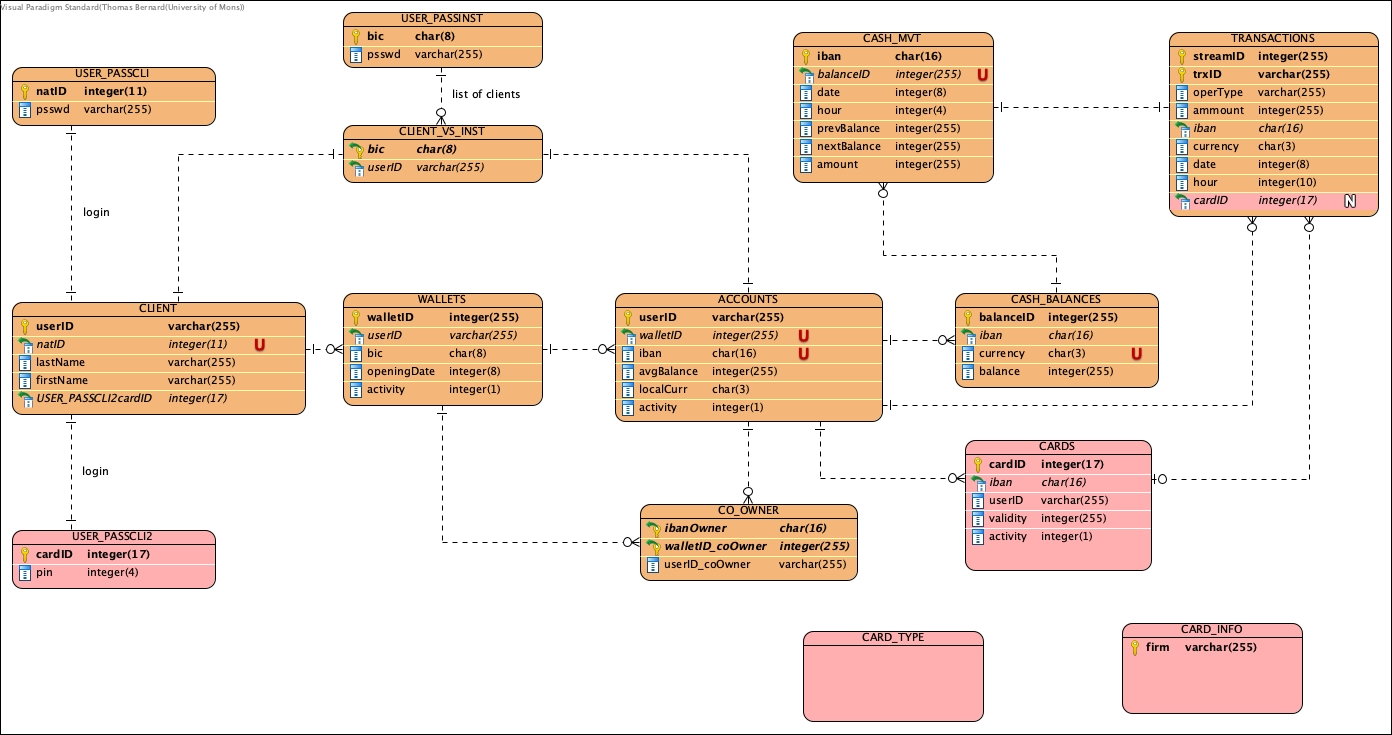
\includegraphics[scale=0.15]{ressources/photos_diagrammes/extensionTheo/erdTheo.jpg}
	\end{figure}

\newpage

\end{document}
